\section{Implementarea lucrarii de laborator}

\subsection{Taskurile implementate}

\begin{itemize}
\item Realizarea unui mini sait cu pagini statice
\item Familiarizarea cu HTML si CSS
\item Interactiuni Javascript
\end{itemize}

\subsection{Analiza lucrarii de laborator}
Repozitoriu pe github.

\subsection{Realizarea unui mini sait }

In acest laborator a fost realizat un sait cu tematica sportului, care presupune mai 
multe pagini statice.
Este un sait de prezentare, ce presupune text formatat, imagini, toggle-box.


\begin{figure}[!ht]
                     \centering
                     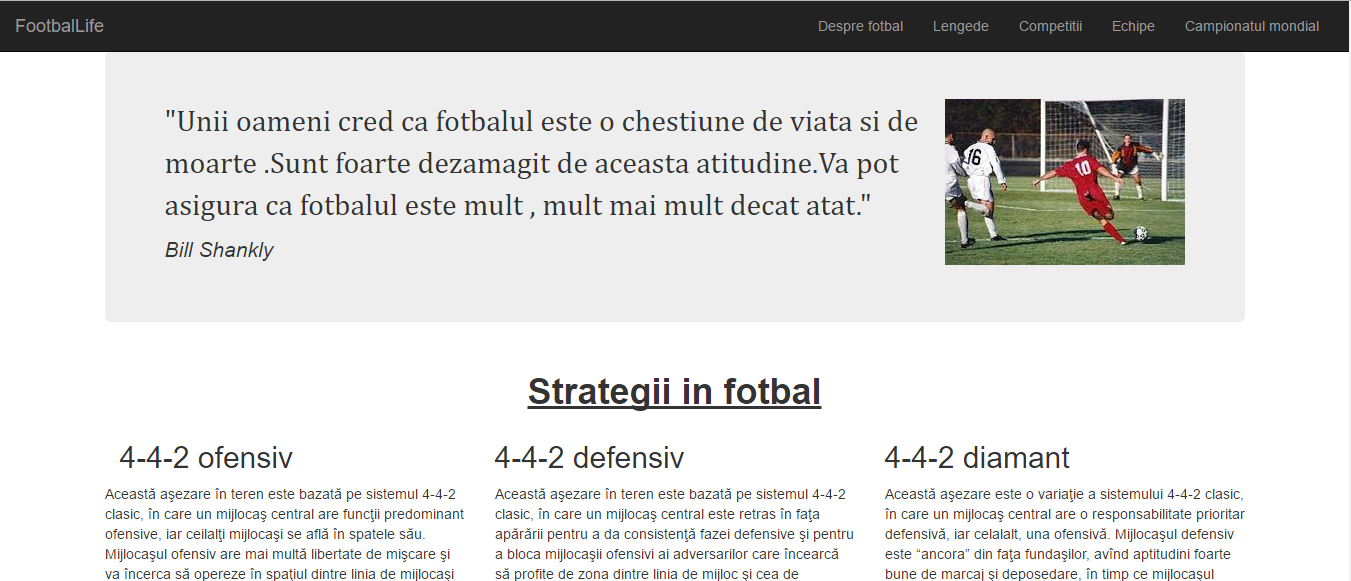
\includegraphics[scale = 0.6]{index}
                     \caption{Pagina principala, \cite{ImRef}}
                     \label{Im_label}
                \end{figure}

\break
Designul elementelor a fost executat in CSS3 si deasemenea implementind 
framework-ul pentru design Bootstrap 3.

Deasemenea saitul contine un element mobil numit carousel, care la un anummit 
interval de timp deruleaza niste imagini.
\begin{figure}[!ht]
                     \centering
                     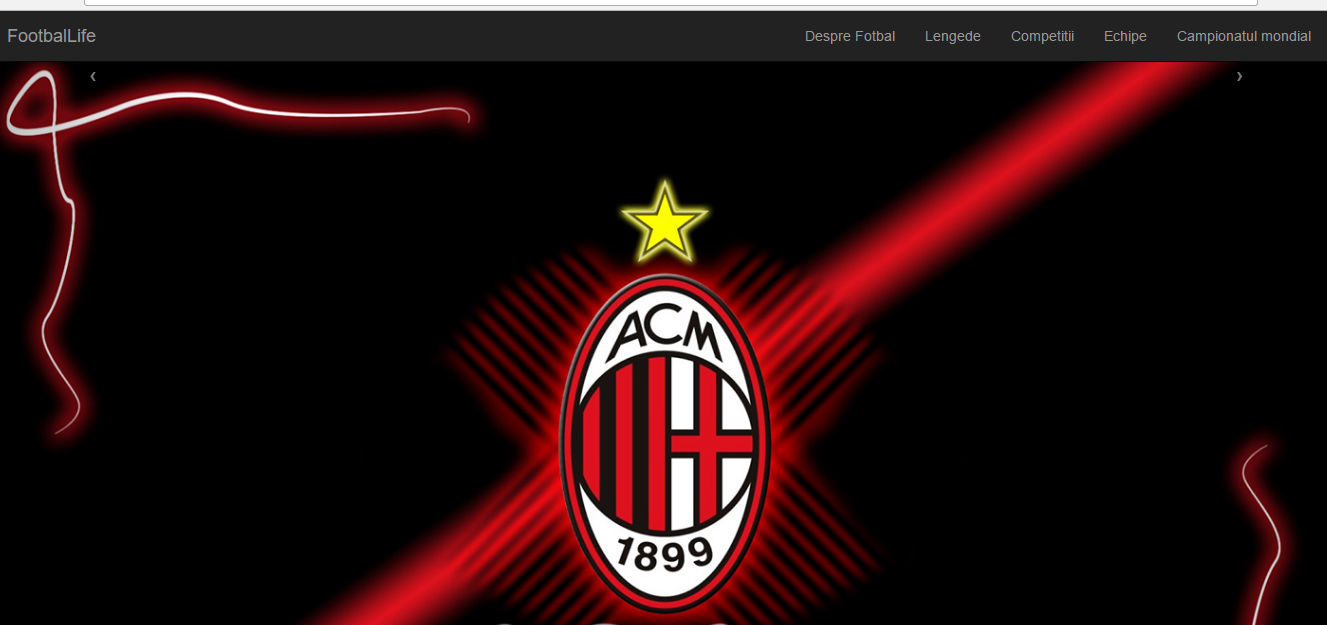
\includegraphics[scale = 0.6]{carousel}
                     \caption{Carousel, \cite{ImRef}}
                     \label{Im_label}
                \end{figure}

Saitul are proprietatea responsive, ceea ce permite vizualizarea de pe device-uri mobile 
fara nici o problema si adaptare la ecran foarte comoda.
Aceasta functionalitate se datoreaza Bootstrap.

\begin{figure}[!ht]
                     \centering
                     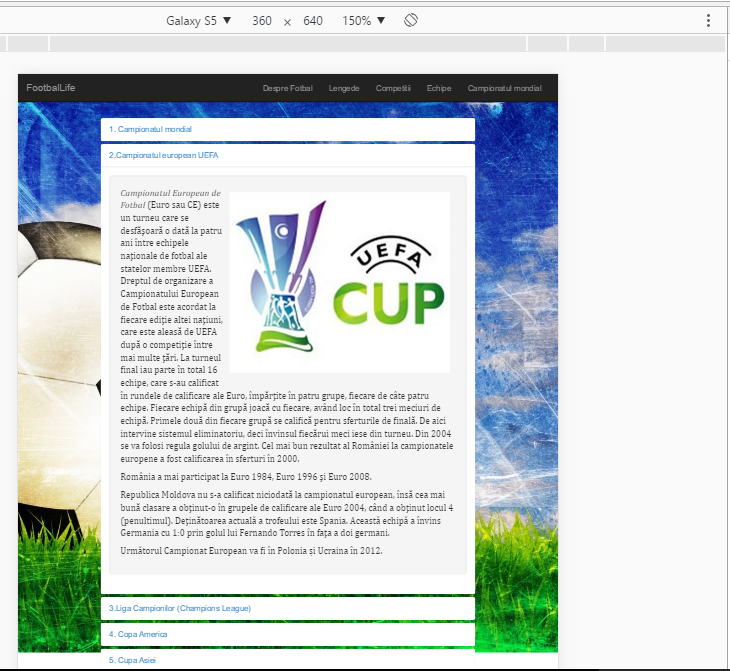
\includegraphics[scale = 0.6]{responsive}
                     \caption{Pagina vizualizata de pe Galaxy S5, \cite{ImRef}}
                     \label{Im_label}
                \end{figure}


\clearpage